% Options for packages loaded elsewhere
\PassOptionsToPackage{unicode}{hyperref}
\PassOptionsToPackage{hyphens}{url}
\PassOptionsToPackage{dvipsnames,svgnames,x11names}{xcolor}
%
\documentclass[
  letterpaper,
  DIV=11,
  numbers=noendperiod]{scrartcl}

\usepackage{amsmath,amssymb}
\usepackage{lmodern}
\usepackage{iftex}
\ifPDFTeX
  \usepackage[T1]{fontenc}
  \usepackage[utf8]{inputenc}
  \usepackage{textcomp} % provide euro and other symbols
\else % if luatex or xetex
  \usepackage{unicode-math}
  \defaultfontfeatures{Scale=MatchLowercase}
  \defaultfontfeatures[\rmfamily]{Ligatures=TeX,Scale=1}
\fi
% Use upquote if available, for straight quotes in verbatim environments
\IfFileExists{upquote.sty}{\usepackage{upquote}}{}
\IfFileExists{microtype.sty}{% use microtype if available
  \usepackage[]{microtype}
  \UseMicrotypeSet[protrusion]{basicmath} % disable protrusion for tt fonts
}{}
\makeatletter
\@ifundefined{KOMAClassName}{% if non-KOMA class
  \IfFileExists{parskip.sty}{%
    \usepackage{parskip}
  }{% else
    \setlength{\parindent}{0pt}
    \setlength{\parskip}{6pt plus 2pt minus 1pt}}
}{% if KOMA class
  \KOMAoptions{parskip=half}}
\makeatother
\usepackage{xcolor}
\setlength{\emergencystretch}{3em} % prevent overfull lines
\setcounter{secnumdepth}{5}
% Make \paragraph and \subparagraph free-standing
\ifx\paragraph\undefined\else
  \let\oldparagraph\paragraph
  \renewcommand{\paragraph}[1]{\oldparagraph{#1}\mbox{}}
\fi
\ifx\subparagraph\undefined\else
  \let\oldsubparagraph\subparagraph
  \renewcommand{\subparagraph}[1]{\oldsubparagraph{#1}\mbox{}}
\fi


\providecommand{\tightlist}{%
  \setlength{\itemsep}{0pt}\setlength{\parskip}{0pt}}\usepackage{longtable,booktabs,array}
\usepackage{calc} % for calculating minipage widths
% Correct order of tables after \paragraph or \subparagraph
\usepackage{etoolbox}
\makeatletter
\patchcmd\longtable{\par}{\if@noskipsec\mbox{}\fi\par}{}{}
\makeatother
% Allow footnotes in longtable head/foot
\IfFileExists{footnotehyper.sty}{\usepackage{footnotehyper}}{\usepackage{footnote}}
\makesavenoteenv{longtable}
\usepackage{graphicx}
\makeatletter
\def\maxwidth{\ifdim\Gin@nat@width>\linewidth\linewidth\else\Gin@nat@width\fi}
\def\maxheight{\ifdim\Gin@nat@height>\textheight\textheight\else\Gin@nat@height\fi}
\makeatother
% Scale images if necessary, so that they will not overflow the page
% margins by default, and it is still possible to overwrite the defaults
% using explicit options in \includegraphics[width, height, ...]{}
\setkeys{Gin}{width=\maxwidth,height=\maxheight,keepaspectratio}
% Set default figure placement to htbp
\makeatletter
\def\fps@figure{htbp}
\makeatother
\newlength{\cslhangindent}
\setlength{\cslhangindent}{1.5em}
\newlength{\csllabelwidth}
\setlength{\csllabelwidth}{3em}
\newlength{\cslentryspacingunit} % times entry-spacing
\setlength{\cslentryspacingunit}{\parskip}
\newenvironment{CSLReferences}[2] % #1 hanging-ident, #2 entry spacing
 {% don't indent paragraphs
  \setlength{\parindent}{0pt}
  % turn on hanging indent if param 1 is 1
  \ifodd #1
  \let\oldpar\par
  \def\par{\hangindent=\cslhangindent\oldpar}
  \fi
  % set entry spacing
  \setlength{\parskip}{#2\cslentryspacingunit}
 }%
 {}
\usepackage{calc}
\newcommand{\CSLBlock}[1]{#1\hfill\break}
\newcommand{\CSLLeftMargin}[1]{\parbox[t]{\csllabelwidth}{#1}}
\newcommand{\CSLRightInline}[1]{\parbox[t]{\linewidth - \csllabelwidth}{#1}\break}
\newcommand{\CSLIndent}[1]{\hspace{\cslhangindent}#1}

\usepackage{amsmath}
\usepackage{booktabs}
\usepackage{caption}
\usepackage{longtable}
\KOMAoption{captions}{tableheading}
\makeatletter
\makeatother
\makeatletter
\makeatother
\makeatletter
\@ifpackageloaded{caption}{}{\usepackage{caption}}
\AtBeginDocument{%
\ifdefined\contentsname
  \renewcommand*\contentsname{Table of contents}
\else
  \newcommand\contentsname{Table of contents}
\fi
\ifdefined\listfigurename
  \renewcommand*\listfigurename{List of Figures}
\else
  \newcommand\listfigurename{List of Figures}
\fi
\ifdefined\listtablename
  \renewcommand*\listtablename{List of Tables}
\else
  \newcommand\listtablename{List of Tables}
\fi
\ifdefined\figurename
  \renewcommand*\figurename{Figure}
\else
  \newcommand\figurename{Figure}
\fi
\ifdefined\tablename
  \renewcommand*\tablename{Table}
\else
  \newcommand\tablename{Table}
\fi
}
\@ifpackageloaded{float}{}{\usepackage{float}}
\floatstyle{ruled}
\@ifundefined{c@chapter}{\newfloat{codelisting}{h}{lop}}{\newfloat{codelisting}{h}{lop}[chapter]}
\floatname{codelisting}{Listing}
\newcommand*\listoflistings{\listof{codelisting}{List of Listings}}
\makeatother
\makeatletter
\@ifpackageloaded{caption}{}{\usepackage{caption}}
\@ifpackageloaded{subcaption}{}{\usepackage{subcaption}}
\makeatother
\makeatletter
\@ifpackageloaded{tcolorbox}{}{\usepackage[many]{tcolorbox}}
\makeatother
\makeatletter
\@ifundefined{shadecolor}{\definecolor{shadecolor}{rgb}{.97, .97, .97}}
\makeatother
\makeatletter
\makeatother
\ifLuaTeX
  \usepackage{selnolig}  % disable illegal ligatures
\fi
\IfFileExists{bookmark.sty}{\usepackage{bookmark}}{\usepackage{hyperref}}
\IfFileExists{xurl.sty}{\usepackage{xurl}}{} % add URL line breaks if available
\urlstyle{same} % disable monospaced font for URLs
\hypersetup{
  pdftitle={Supplementary material},
  colorlinks=true,
  linkcolor={blue},
  filecolor={Maroon},
  citecolor={Blue},
  urlcolor={Blue},
  pdfcreator={LaTeX via pandoc}}

\title{Supplementary material}
\author{}
\date{}

\begin{document}
\maketitle
\begin{abstract}
This document uses a reproductible workflows to provide descriptive
statistics to the scientific papers it accompanies. In section 1 we
briefly present the technical setting used for these calculation and
explain how they make it possible for reviewers and researches to verify
and reproduce these calculations. In section 2, we analyse the world
database on protected areas to assess how the relative importance of
multipurpose protected areas has evolved compared to strictly protected
areas. In section 3, we analyse the database on protected areas
management evaluations to assess the absolute and relative importance of
evaluation methods by type of countries.
\end{abstract}
\ifdefined\Shaded\renewenvironment{Shaded}{\begin{tcolorbox}[boxrule=0pt, borderline west={3pt}{0pt}{shadecolor}, interior hidden, enhanced, breakable, sharp corners, frame hidden]}{\end{tcolorbox}}\fi

\hypertarget{technical-settings}{%
\section{Technical settings}\label{technical-settings}}

This document is designed to provide a verifiable and reproducible
answer to this question. It is written in
\href{https://quarto.org/}{quarto} and uses R code. All the data
processing can be viewed by clicking on the ``code'' buttons.

\hypertarget{trends-in-protected-area-types-by-period-of-establishment}{%
\section{Trends in protected area types by period of
establishment}\label{trends-in-protected-area-types-by-period-of-establishment}}

\hypertarget{objective}{%
\subsection{Objective}\label{objective}}

We want to know if the share of multi-purpose protected areas is
increasing, compared to protected areas pursuing only conservation
objectives. We show very different trends whether we focus on the number
of entities or the spatial coverage of protected areas.

\hypertarget{data}{%
\subsection{Data}\label{data}}

We use the extension wdpar to fetch the World Database on Protected
Areas from \href{https://www.protectedplanet.net/en}{the protected
planet portal}. It is the version updated in February 2022. We only keep
the areas for which a spatial area is known, that is not including the
protected area for which only one point in space is reported.

As of this date, the WDPA includes information on
\texttt{rnrow(wdpa\_gee)} protected areas. A well-formatted description
of the fields available can be found
\href{https://developers.google.com/earth-engine/datasets/catalog/WCMC_WDPA_current_polygons}{on
this webpage}.

\hypertarget{methods}{%
\subsection{Methods}\label{methods}}

We keep only terrestrial protected areas and discard marine or coastal
protected areas. There is no consensus on IUCN categories in the
literature. Ellason et al. (2021) suggest the following classification,
which we complement here with the naming used by the authors:

\begin{itemize}
\item
  Some studies group I and II in one class, and all others in another
  class:

  \begin{itemize}
  \item
    Sharlemann et al. (2010) classify cat. I and II as ``protected sites
    with more restrictive land management regimes'' and III to VI as
    ``all other protected sites''
  \item
    Jones et al. (2018) designate I and II as ``strict biodiversity
    conservation areas'' and III to VI as ``zones permitting certain
    human activities and sustainable resource extraction''
  \item
    Anderson and Mammides (2020) designate only I and II as ``areas in
    stricter categories''.
  \end{itemize}
\item
  Other studies group I, II and III in one class, and IV, V and VI in
  another class:

  \begin{itemize}
  \item
    Seiferling et al. (2012) designate I to III as ``areas into
    high-protection'' and IV to VI as ``low protection categories''.
  \item
    Françoso et al. (2015) refer to IV to VI as ``sustainable use PAs''
    and the other as ``other''.
  \end{itemize}
\item
  Other studies group I to IV in one class and V and VI in another
  class:

  \begin{itemize}
  \item
    Nelson and Chomitz (2011) refer to I to IV as ``strict protection''
    and V and VI as ``nonstrict or multi-use protection''.
  \item
    Porter-Bordland et al. (2012) refer as I to IV as ``protected
    areas'' and V and VI as ``community managed forests''.
  \end{itemize}
\end{itemize}

Adding to this classification, we share Ledberger (2020) analysis that
classifies the naturalness of IUCN category definition as follows: Ia =
Ib \textgreater{} II = III \textgreater{} IV = VI \textgreater{} V and
they find out that ``the global ranking of the effect of the IUCN
categories on the forest loss per PA at the global scale, from the least
to the most forest loss, was III \textless{} Ia = Ib = II \textless{} IV
= V = VI'' .

We consider that Lebergers et al.~results (2020) convincingly make the
case to group I to III. We find out however that vivid debates focused
on the category IV definition and revision (Leroux et al. 2010), so keep
IV separated in our analysis, its purpose and criteria are different
from V and VI\footnote{From the literature, we could even consider also
  separating III in a separate category, to have 3 classes: I-II, III,
  IV and V-VI.}.

After this filtering, we have 225411 protected areas for the analysis.

\hypertarget{results}{%
\subsection{Results}\label{results}}

\hypertarget{relative-importance-of-status-in-number-of-pas}{%
\subsubsection{Relative importance of status in number of
PAs}\label{relative-importance-of-status-in-number-of-pas}}

Figure~\ref{fig-n-pas} represents the evolution of strict
vs.~multipurpose categories according to the year of assignment of the
conservation status of PAs.

\begin{figure}

{\centering 
\includegraphics{Suppl_material_test_EoH_files/figure-pdf/fig-n-pas-1.pdf}

}

\caption{\label{fig-n-pas}Number of terrestrial protected areas by
status and decade of creation (source: WDPA, Jan.~2023)}

\end{figure}

The Figure~\ref{fig-n-pas} shows that the total number of PAs has
sharply increased since 2000. However, the relative importance of
multipurpose conservation status doesn't seem to increase.

\hypertarget{tbl-npas}{}
\begin{longtable}{crrrrrrrrr}
\caption{\label{tbl-npas}Area of PAs by status category and decade of creation (source: WDPA,
Jan. 2023) }\tabularnewline

\toprule
Decade of status assignment & IV & Nonstrict & Strict & Unknown & Total number of PAs created & Number of PAs whith a known status & \% of strict among known status & \% of IV among known status & \% of multipurpose among known status \\ 
\midrule
Before 1960 & 1833 & 2118 & 1825 & 1568 & 7344 & 5776 & 31.6 & 31.7 & 36.7 \\ 
1960-1969 & 1612 & 1639 & 1236 & 1446 & 5933 & 4487 & 27.5 & 35.9 & 36.5 \\ 
1970-1979 & 3246 & 3068 & 2900 & 1190 & 10404 & 9214 & 31.5 & 35.2 & 33.3 \\ 
1980-1989 & 9801 & 3784 & 7859 & 1851 & 23295 & 21444 & 36.6 & 45.7 & 17.6 \\ 
1990-1999 & 14593 & 7589 & 8598 & 5573 & 36353 & 30780 & 27.9 & 47.4 & 24.7 \\ 
2000-2009 & 23579 & 10972 & 8306 & 25239 & 68096 & 42857 & 19.4 & 55.0 & 25.6 \\ 
2010-2019 & 23797 & 6729 & 6392 & 28314 & 65232 & 36918 & 17.3 & 64.5 & 18.2 \\ 
2020-2029 & 1631 & 494 & 911 & 5718 & 8754 & 3036 & 30.0 & 53.7 & 16.3 \\ 
\bottomrule
\end{longtable}

For readability purpose, we present the proportions displayed in the
three last column of the table above in the figure below.

\begin{figure}

{\centering 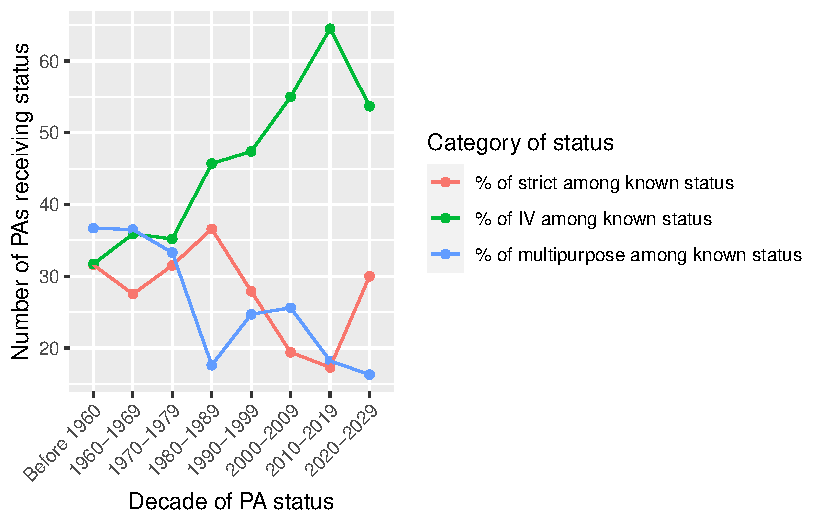
\includegraphics{Suppl_material_test_EoH_files/figure-pdf/fig-prop-pas-n-1.pdf}

}

\caption{\label{fig-prop-pas-n}Proportion of terrestrial PAs by status
and decade of creation (source: WDPA, Jan.~2023)}

\end{figure}

According to the world database on protected areas, the proportion of
new protected areas with a multipurpose status has reduced, from 36.5\%
in the 1960s to 18.2\% in the 2010s. It has been even lower (16.3\%) in
the first years of the current decade.

We must, however, strikeout that the decade of creation is unknown for
out of 225411 protected area ( \%). There is a large proportion of
multipurpose status among the protected areas for which the creation
date is unknown (\%). The status of the protected area is unknown for
70899 protected areas out of 225411 protected areas (31.5\%).

\hypertarget{relative-importance-of-status-in-pa-spatial-extent}{%
\subsubsection{Relative importance of status in PA spatial
extent}\label{relative-importance-of-status-in-pa-spatial-extent}}

We now perform the same analysis, but instead of counting the number of
PAs, we sum their area. The area newly covered by type of status is
represented in Figure~\ref{fig-area-pas}.

\begin{figure}

{\centering 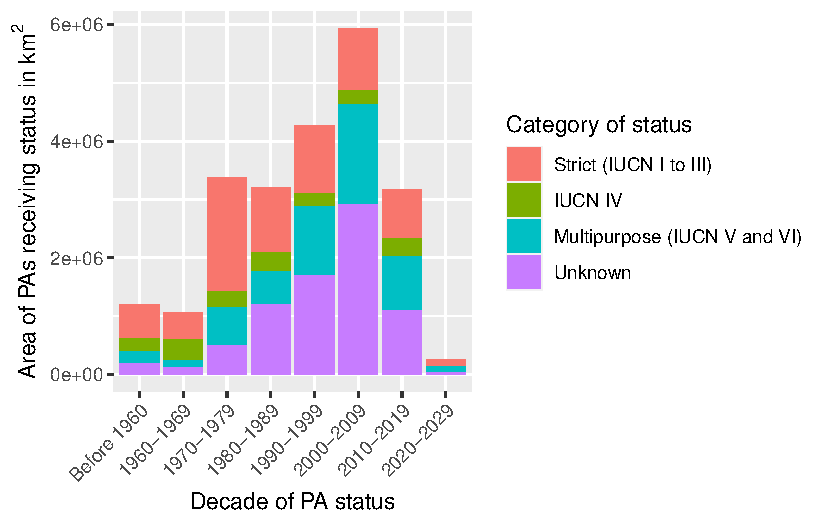
\includegraphics{Suppl_material_test_EoH_files/figure-pdf/fig-area-pas-1.pdf}

}

\caption{\label{fig-area-pas}Area of terrestrial protected areas by
status and decade of creation (source: WDPA, Jan.~2023)}

\end{figure}

The trend that appears in Figure~\ref{fig-area-pas} is quite different
than the one we saw in Figure~\ref{fig-n-pas}: when accounting for their
total areas, multi-purpose protected areas seem to represent an
increasing proportion among newly created protected areas.

We now compute the precise area estimates and their relative importance.

\hypertarget{tbl-area-pas}{}
\begin{longtable}{crrrrr}
\caption{\label{tbl-area-pas}Area of terrestrial protected areas by status and decade of creation
(source: WDPA, Jan. 2023) }\tabularnewline

\caption*{
{\large Area of terrestrial protected areas by status and decade of creation (source: WDPA, Jan. 2023)}
} \\ 
\toprule
Decade of status assignment & Total number of PAs created & Area of PAs whith a known status & \% of strict among known status & \% of IV among known status & \% of multipurpose among known status \\ 
\midrule
Before 1960 & 1204871 & 1014137 & 56.1 & 23.7 & 20.1 \\ 
1960-1969 & 1065311 & 950917 & 46.6 & 40.3 & 13.1 \\ 
1970-1979 & 3375221 & 2877048 & 67.1 & 10.1 & 22.8 \\ 
1980-1989 & 3213364 & 2012967 & 55.2 & 16.8 & 28.0 \\ 
1990-1999 & 4261764 & 2571630 & 44.3 & 9.2 & 46.5 \\ 
2000-2009 & 5927647 & 3016458 & 34.7 & 8.5 & 56.8 \\ 
2010-2019 & 3168746 & 2068334 & 39.5 & 16.2 & 44.3 \\ 
2020-2029 & 259555 & 217955 & 50.1 & 3.7 & 46.2 \\ 
\bottomrule
\end{longtable}

The same information, in graphics:

\begin{figure}

{\centering 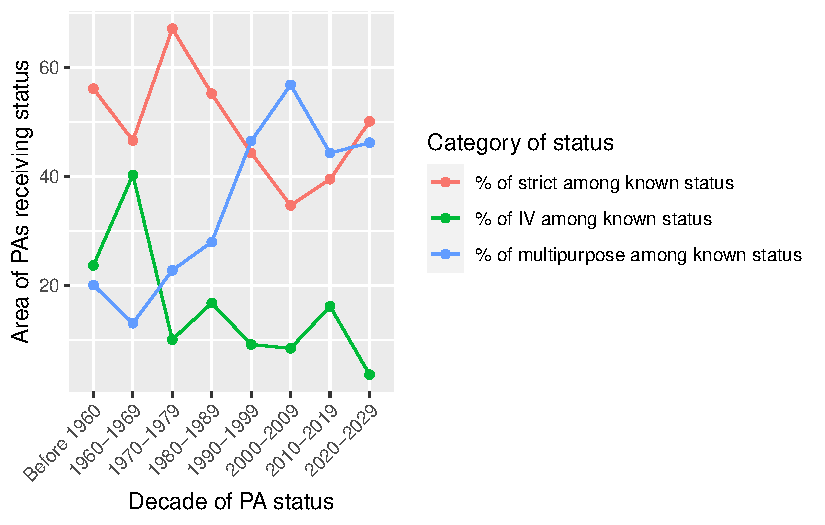
\includegraphics{Suppl_material_test_EoH_files/figure-pdf/fig-prop-pas_area-1.pdf}

}

\caption{\label{fig-prop-pas_area}Relative area of terrestrial PAs by
status and decade of creation (source: WDPA, Jan.~2023)}

\end{figure}

According to the world database on protected areas, the total spatial
extent of new protected areas with a multipurpose status has increased,
from 13.1\% in the 1960s to 56.8\% in the 2000s and slightly decreased
in the 2010s to 44.3\%.

\hypertarget{average-size-of-protected-areas}{%
\subsubsection{Average size of protected
areas}\label{average-size-of-protected-areas}}

The two previous figures suggest very different trends in terms of
average size of protected areas depending on their status. We verify
this with Figure~\ref{fig-avg-area}.

\begin{figure}

{\centering 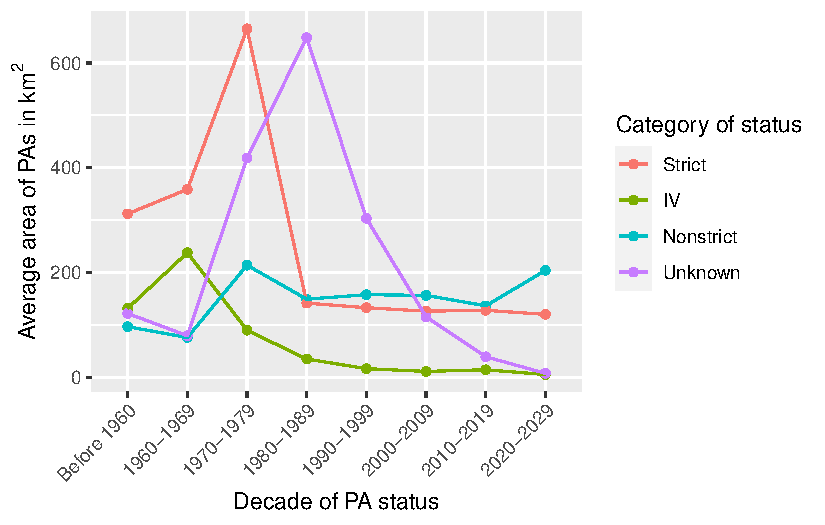
\includegraphics{Suppl_material_test_EoH_files/figure-pdf/fig-avg-area-1.pdf}

}

\caption{\label{fig-avg-area}Average area of terrestrial protected areas
by status and decade of creation (source: WPDA, Jan.~2023)}

\end{figure}

Figure~\ref{fig-avg-area} shows that the area of PAs with a strict
status has decreased over time, while the area of PAs with a
multipurpose status has increased over time. The protected area of
category have dramatically shrinked and are now very small.

\hypertarget{total-size-of-protected-areas}{%
\subsection{Total size of protected
areas}\label{total-size-of-protected-areas}}

Summing up the total area of protected areas by type, we obtain the
following proportions.

\hypertarget{tbl-prop-tot}{}
\begin{longtable}{lrrrr}
\caption{\label{tbl-prop-tot}Relative importance of PA types among PAs for which status is documented
(source: WDPA, Fev. 2023) }\tabularnewline

\caption*{
{\large Relative importance of PA types among PAs for which status is documented (source: WDPA, Fev. 2023)}
} \\ 
\toprule
Type d'aire protégée & Number of PAs & \% in number of PAs & Total area in km<sup>2</sup> & \% in area \\ 
\midrule
Strict (IUCN I to IV) & 38027 & 24.61 & 7166153 & 48.65 \\ 
IUCN IV & 80092 & 51.84 & 2089144 & 14.18 \\ 
Multipurpose (IUCN V and VI) & 36393 & 23.55 & 5474149 & 37.16 \\ 
\bottomrule
\end{longtable}

\hypertarget{conclusion}{%
\subsection{Conclusion}\label{conclusion}}

The information available in the world database on protected areas
indicates that \textbf{in terms of number of administrative entities},
the proportion protected areas with a multi-purpose status tends to
decrease over the last decades. However, \textbf{in terms of spatial
extent of these entities},the proportion of protected area with a
multi-purpose status tends to increase over the same period. In other
words, countries create an increasing number of smaller strictly
protected areas, and they create a decreasing number of larger
multi-purpose protected areas. Protected areas of category IV have a
very ambiguous status and their trend clearly stand out, as their their
number among newly created protected areas has doubled, while their
relative area has shrinked.

This conclusion, however, could be undermined by the substantial
proportion of missing information on the creation date and status of
protected areas in the database of reference.

\hypertarget{usage-of-pame-methods-by-country-income-group}{%
\section{Usage of PAME methods by country income
group}\label{usage-of-pame-methods-by-country-income-group}}

\hypertarget{objective-1}{%
\subsection{Objective}\label{objective-1}}

We want to assess the prevalence of METT and RAPPAM methodologies among
PAMEs, depending of the country income group. We show that method usages
are very different in high income countries in comparison to medium and
low income countries.

\hypertarget{data-1}{%
\subsection{Data}\label{data-1}}

We download the DB-PAME from the from
\href{https://pame.protectedplanet.net/}{the protected planet portal}.
It is the version updated in February 2022.

We download the World Bank country classification from the World bank
data portal. The data comes in four classes: low income countries, low
medium income countries and high medium income countries. The
classification is available for all years since 1989.

Income status is missing for about a fourth of the countries at the
beginning of the period (in particular countries from the ex soviet
block). It is missing for less than 10 countries (\textless4\%) since
2010.

\hypertarget{results-1}{%
\subsection{Results}\label{results-1}}

We summarise the PAME production by income category of countries and by
group of methods.

\begin{longtable}{lrrrr}
\caption{Prevalance of METT and RAPAM in PAME (source: DB-PAME, Feb. 2023)}\tabularnewline

\toprule
County income category & Number of countries & Total number of assessments & METT or RAPPAM (\%) & Other methods (\%) \\ 
\midrule
Low income & 25 & 778 & 59.25 & 40.36 \\ 
Lower middle income & 47 & 1828 & 66.96 & 32.49 \\ 
Upper middle income & 47 & 3901 & 68.96 & 30.94 \\ 
All low and middle income income & 119 & 6507 & 67.24 & 32.50 \\ 
Low income & 51 & 20390 & 2.94 & 97.05 \\ 
\bottomrule
\end{longtable}

From the results above, we can conclude that most of PAME registered in
the DB-PAME occured in high income countries. We can also observe that
METT and RAPPAM methods are dominant in LMIC, while they remain very
marginal in developping countries.

\hypertarget{references-cited-in-the-supplementaty-material-section}{%
\section*{References cited in the supplementaty material
section}\label{references-cited-in-the-supplementaty-material-section}}
\addcontentsline{toc}{section}{References cited in the supplementaty
material section}

\hypertarget{refs}{}
\begin{CSLReferences}{1}{0}
\leavevmode\vadjust pre{\hypertarget{ref-anderson2020}{}}%
Anderson, Emily, and Christos Mammides. 2020. {``The Role of Protected
Areas in Mitigating Human Impact in the World{'}s Last Wilderness
Areas.''} \emph{Ambio} 49 (2): 434--41.
\url{https://doi.org/10.1007/s13280-019-01213-x}.

\leavevmode\vadjust pre{\hypertarget{ref-elleason2021}{}}%
Elleason, Moses, Zhuoli Guan, Yiming Deng, Aiwu Jiang, Eben Goodale, and
Christos Mammides. 2021. {``Strictly Protected Areas Are Not Necessarily
More Effective Than Areas in Which Multiple Human Uses Are Permitted.''}
\emph{Ambio} 50 (5): 1058--73.
\url{https://doi.org/10.1007/s13280-020-01426-5}.

\leavevmode\vadjust pre{\hypertarget{ref-franuxe7oso2015}{}}%
Françoso, Renata D., Reuber Brandão, Cristiano C. Nogueira, Yuri B.
Salmona, Ricardo Bomfim Machado, and Guarino R. Colli. 2015. {``Habitat
Loss and the Effectiveness of Protected Areas in the Cerrado
Biodiversity Hotspot.''} \emph{Natureza \& Conservação} 13 (1): 35--40.
\url{https://doi.org/10.1016/j.ncon.2015.04.001}.

\leavevmode\vadjust pre{\hypertarget{ref-jones2018}{}}%
Jones, Kendall R., Oscar Venter, Richard A. Fuller, James R. Allan, Sean
L. Maxwell, Pablo Jose Negret, and James E. M. Watson. 2018.
{``One-Third of Global Protected Land Is Under Intense Human
Pressure.''} \emph{Science} 360 (6390): 788--91.
\url{https://doi.org/10.1126/science.aap9565}.

\leavevmode\vadjust pre{\hypertarget{ref-leberger2020}{}}%
Leberger, Roxanne, Isabel M. D. Rosa, Carlos A. Guerra, Florian Wolf,
and Henrique M. Pereira. 2020. {``Global Patterns of Forest Loss Across
IUCN Categories of Protected Areas.''} \emph{Biological Conservation}
241 (January): 108299.
\url{https://doi.org/10.1016/j.biocon.2019.108299}.

\leavevmode\vadjust pre{\hypertarget{ref-leroux2010}{}}%
Leroux, Shawn J., Meg A. Krawchuk, Fiona Schmiegelow, Steven G. Cumming,
Kim Lisgo, Lee G. Anderson, and Mirela Petkova. 2010. {``Global
Protected Areas and IUCN Designations: Do the Categories Match the
Conditions?''} \emph{Biological Conservation} 143 (3): 609616.

\leavevmode\vadjust pre{\hypertarget{ref-nelson2011}{}}%
Nelson, Andrew, and Kenneth M. Chomitz. 2011. {``Effectiveness of Strict
Vs. Multiple Use Protected Areas in Reducing Tropical Forest Fires: A
Global Analysis Using Matching Methods.''} Edited by Hans Henrik Bruun.
\emph{PLoS ONE} 6 (8): e22722.
\url{https://doi.org/10.1371/journal.pone.0022722}.

\leavevmode\vadjust pre{\hypertarget{ref-porter-bolland2012}{}}%
Porter-Bolland, Luciana, Edward A. Ellis, Manuel R. Guariguata, Isabel
Ruiz-Mallén, Simoneta Negrete-Yankelevich, and Victoria Reyes-García.
2012. {``Community Managed Forests and Forest Protected Areas: An
Assessment of Their Conservation Effectiveness Across the Tropics.''}
\emph{Forest Ecology and Management}, Multiple Use of Tropical Forests:
From Concept to Reality, 268 (March): 6--17.
\url{https://doi.org/10.1016/j.foreco.2011.05.034}.

\leavevmode\vadjust pre{\hypertarget{ref-scharlemann2010}{}}%
Scharlemann, Jörn P. W., Valerie Kapos, Alison Campbell, Igor Lysenko,
Neil D. Burgess, Matthew C. Hansen, Holly K. Gibbs, Barney Dickson, and
Lera Miles. 2010. {``Securing Tropical Forest Carbon: The Contribution
of Protected Areas to REDD.''} \emph{Oryx} 44 (3): 352--57.
\url{https://doi.org/10.1017/S0030605310000542}.

\leavevmode\vadjust pre{\hypertarget{ref-seiferling2012}{}}%
Seiferling, Ian S., Raphaël Proulx, Pedro R. Peres-Neto, Lenore Fahrig,
and Christian Messier. 2012. {``Measuring Protected-Area Isolation and
Correlations of Isolation with Land-Use Intensity and Protection
Status.''} \emph{Conservation Biology} 26 (4): 610--18.
\url{https://doi.org/10.1111/j.1523-1739.2011.01674.x}.

\end{CSLReferences}



\end{document}
